\documentclass[]{beamer}%\documentclass[draft]{beamer}
\mode<presentation>
{
	\usetheme{Madrid}
	\usecolortheme{beaver}
}

\usepackage[utf8]{inputenc}
\usepackage{graphicx}
\usepackage{hyperref}
\usepackage[export]{adjustbox}

\title[About presentation] %optional
{Box2D Project Report Presentation}
\author{
	B Srinivas \\
   \texttt{Roll No. 140050064
    bsrinivasnaik@gmail.com}\\
\and
	KM Mugilvannan \\
    \texttt{Roll No. 140050083 
    vannan1997@gmail.com}\\
\and
	B Gowtham \\
    \texttt{Roll No. 140050085 
    gowtham10896@gmail.com}\\
}
\date{Oct 20, 2015}
\setbeamerfont{fig_font}{size=\small}
\setbeamercovered{invisible}
\usefonttheme[onlysmall]{structurebold}

\begin{document}

\begin{frame}
\titlepage
\end{frame}

\frame{\titlepage}

\begin{frame}
	\frametitle{Overview} 
	\begin{columns}
	\column{0.5\textwidth}	
		\tableofcontents[] 
	\column{0.5\textwidth}	
	\end{columns}
\end{frame}

\begin{frame}
\frametitle{Introduction}
	\begin{itemize}
		\item<1->This project involves using the concepts of box2d to build the rube goldberg simulation which in our case is an interesting monologue between the famous disney characters tom and jerry. 
		\item<2->The difference in this version is that tom gets lucky by trapping jerry with a trap. 
		\item<3->The simulation starts with tom setting one of the dominos off balance and further following the simulation ends where the trap cage shuts jerry out of the outside. 
		\item<4->Here we have assumed that tom already knows the rat burrow which jerry uses as hidden route and uses ray casting to identify the length and time taken by jerry to reach the trap zone and thus setting the simulation accordingly.
	\end{itemize} 
\end{frame}

\begin{frame}
\frametitle{Purpose of this project}
	\begin{itemize}
		\item<1->During the development of this project we had the chance to learn concepts related to makefiles, using abstract c++ implementations in box2d, beamer latex documentation, pdflatex documentation, profiling and debugging and GitHub usage. 
		\item<2->All the box2d implementation contains behind the scene physics engines running which are being annotated in the slides below.
	\end{itemize}
\end{frame}

\section{Body}

\subsection{Part 1: Pendulum}

\begin{frame}
\frametitle{Part 1: Pendulum}
\center
The Formula for the time period of a pendulum is: \pause
\begin{equation}
	T = 2\pi \sqrt {\frac{l}{g}}
\end{equation}
\begin{flushleft}
\begin{itemize}
\pause
\item Here $ l $ is the length of thread from bob to pivot point and $ g $ is the acceleration due to gravity($ \approx 9.81 m/sec^2 $)\pause
\item $ g $ is the acceleration due to gravity.\\ \pause
\item $ v_x $ id the initial velocity of ball in x-direction (No acceleration in x-direction).\pause
\end{itemize}
\end{flushleft}
\begin{figure}
		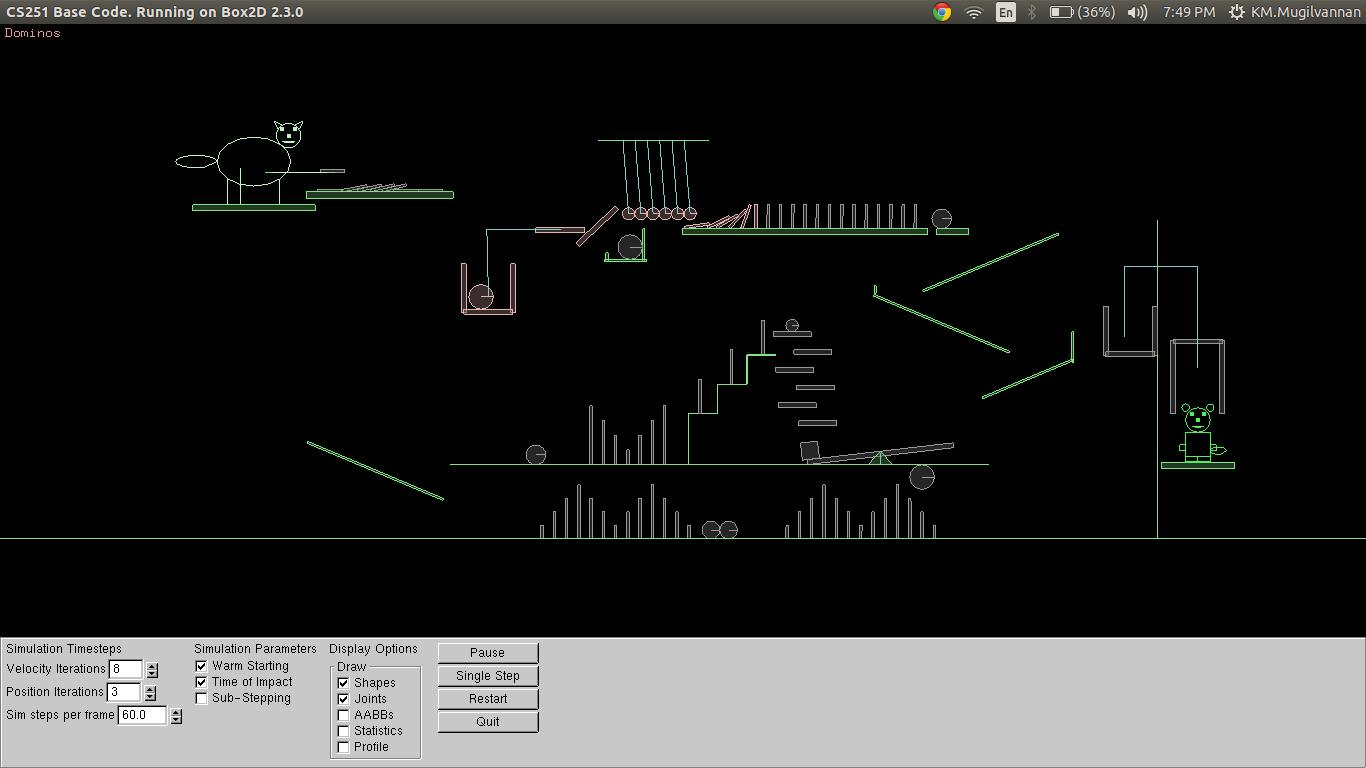
\includegraphics[width=2.5cm,height=2.5cm,keepaspectratio]{Middle.jpg}
\end{figure}
\end{frame}

\subsection{Part 2: Flying Ball}

\begin{frame}
\frametitle{Part 2: Flying Ball}
\center
The equation of motion of a ball in free fall is: \\
\begin{equation}
	s_y = u_y t + \frac{1}{2}gt^2
\end{equation}
\begin{equation}
	s_x = v_x t
\end{equation}
\begin{flushleft}
\begin{itemize}
\item $ s_y $ is the displacement in the y direction and $ s_x $ is the dispacement in x direction.\pause \\
\item $ g $ is the acceleration due to gravity.\pause \\
\item $ v_x $ id the initial velocity of ball in x-direction (No acceleration in x-direction).\pause
\end{itemize}
\end{flushleft}
\begin{figure}
		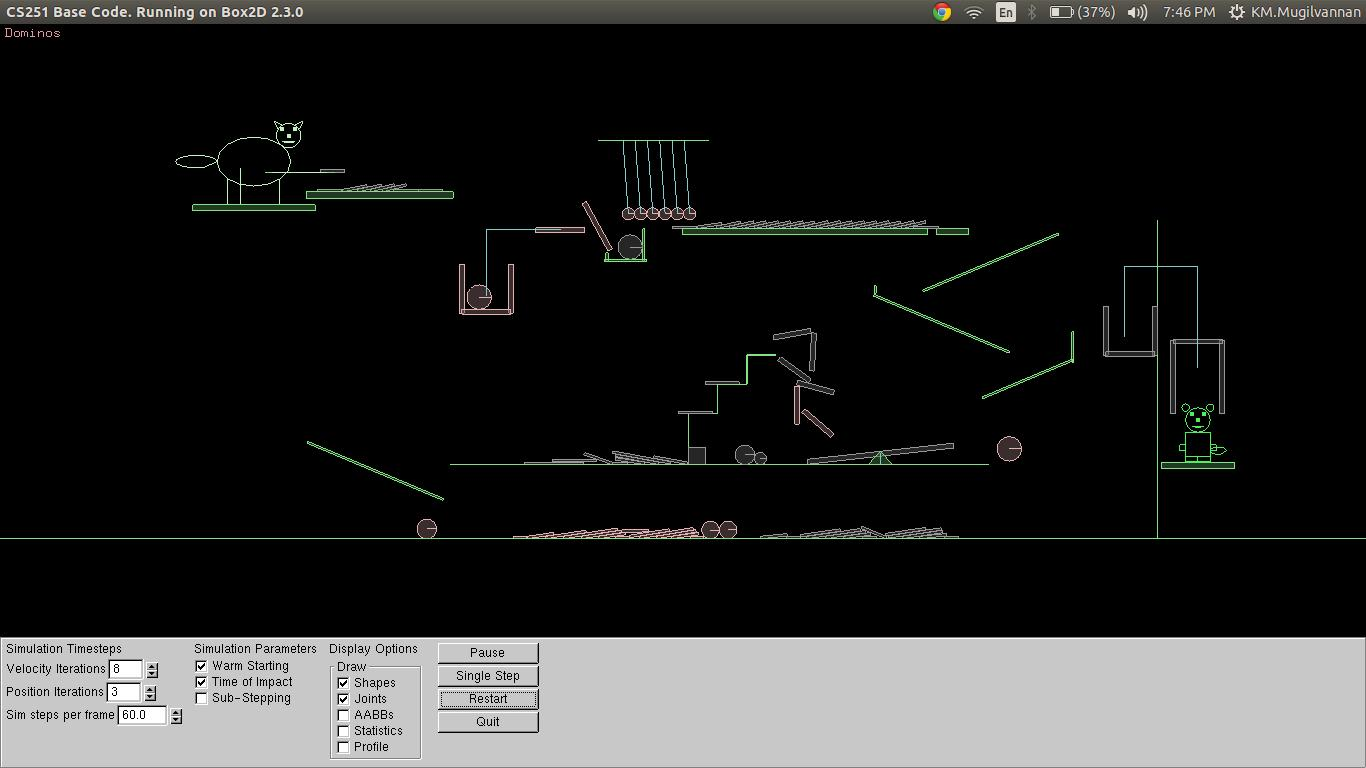
\includegraphics[width=2.5cm,height=2.5cm,keepaspectratio]{Flyball.jpg}
\end{figure}
\end{frame}


\begin{frame}
\frametitle{Final Simulation}
\center
\begin{figure}
	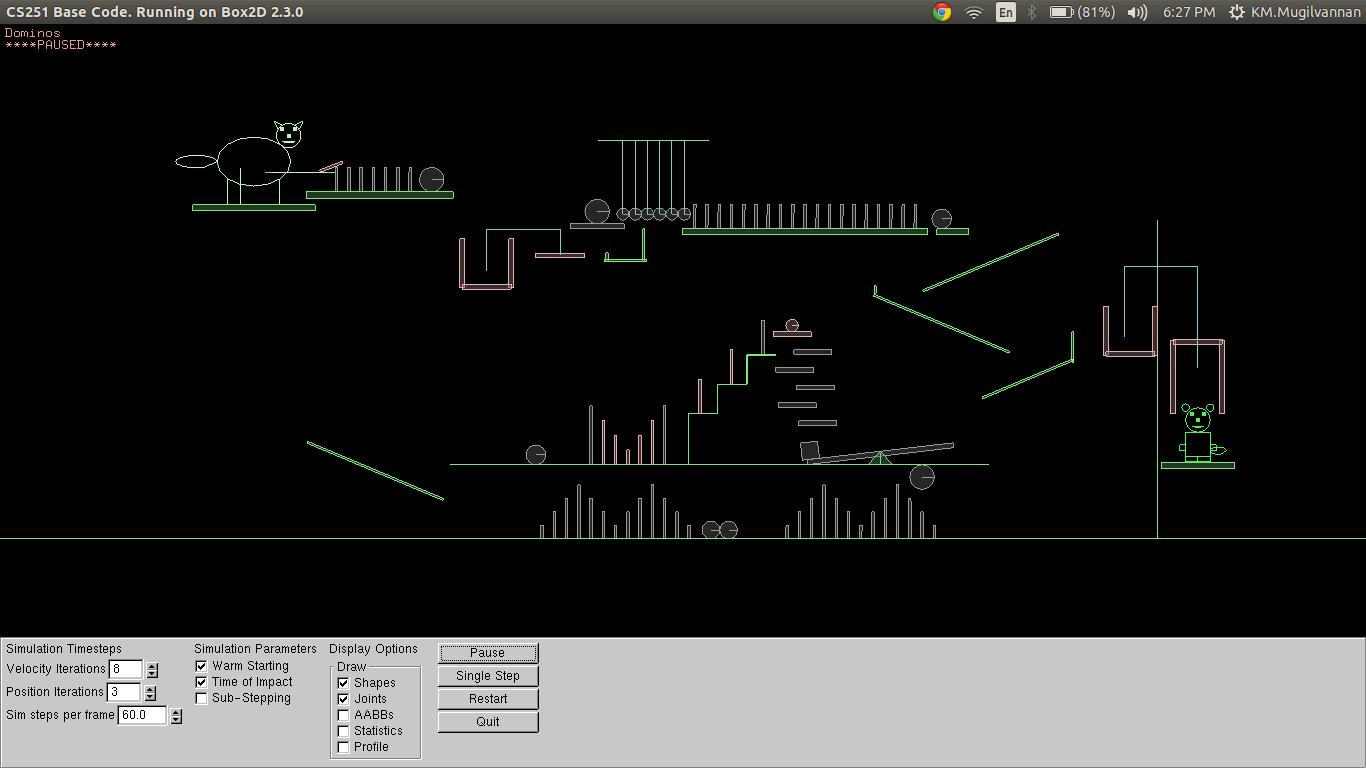
\includegraphics[width=7cm,height=7cm,keepaspectratio]{Toms_turn.jpg}
\end{figure}
\end{frame}

\begin{frame}
\frametitle{Conclusion}
    \begin{itemize}
        \item<1->Helped us learn many concepts as described above
        \item<2->Softwares used to construct the presentation and other reports are far better than the conventional way of representing data and are more efficient.
    \end{itemize}
\end{frame}


\end{document}